% reviewers: Zam, Jared?

% look up Alon 1996 paper from melsted
% ``curse of sequencing'' Roberts 2011, from melsted

% TODO:
% apply to larger data sets - ask Sherine to configure, run, write.
%% examine lousy specificity

% Writing:
% address lousy specificity, viz. streaming trimming

\documentclass{article}
\usepackage{graphicx}
\bibliographystyle{plos2009}


\begin{document}

\title{Streaming approaches to error detection and trimming in the analysis of
short sequencing reads}
\author{TBD}
\maketitle

\section{Introduction}

K-mer spectral analysis is a powerful approach to error detection and
correction in shotgun sequencing data that uses k-mer abundances to
determine likely errors \cite{Pevzner2001}.  Approaches derived from
spectral analysis can be very accurate: Zhang et al. (2014) show that
spectral k-mer trimming is considerably more effective at removing
errors than quality score-based approaches \cite{Zhang2014}.  However,
spectral analysis is also very compute intensive; most implementations
count all the k-mers in sequencing data sets, which can be memory- or
I/O-intensive for large data sets \cite{Zhang2014}.

Streaming algorithms offer improved algorithmic and computational
efficiency in the analysis of large data sets \cite{Charikar2004,
  Cormode2005}.  Streaming algorithms typically examine the data only
once, and have memory usage that scales sublinearly with the size of
the input data.  Streaming algorithms have not been applied to k-mer
spectral analysis of sequencing reads, although Melsted et
al. developed an effective streaming algorithm for calculating
aggregate statistics of k-mer distributions from sequencing data
\cite{Melsted2014}.

Brown et al. (2012) introduced a streaming algorithm for downsampling
read data sets to normalize read coverage spectra, termed ``digital
normalization'' (abbreviated as ``diginorm'') \cite{Brown2012}.  This
procedure estimates the k-mer coverage of each read in a stream using
an online algorithm. Reads above a certain estimated coverage are set
aside and their k-mers are not tracked.  The diginorm algorithm only
examines the data once, and counts only the k-mers in retained reads,
leading to sublinear memory usage for high-coverage data sets
\cite{Brown2012}.

Here we develop a streaming algorithm for k-mer spectral analysis,
based on digital normalization, that can detect and remove errors in
sequencing reads.  This algorithm operates in sublinear memory, and
examines the data at most twice.  The approach offers a general
framework for streaming sequence analysis and could be used for error
correction and variant calling.  Moreover, the approach can be applied
generically to data sets with variable coverage such as
transcriptomes, metagenomes, and amplified genomic DNA.  We also
provide an approach for estimating per-position sequencing error rates
that operates in sublinear time and memory with respect to the input
data.

\section{Results}

\subsection{Coverage-normalized data can be used to locate
and correct errors in high-coverage shotgun sequencing data}

Digital normalization eliminates many erroneous k-mers, while
retaining the majority of true k-mers \cite{Brown2012}.  Our initial
question was whether we could apply spectral error analysis to genomic
short read data after digital normalization.  We tested this on a
synthetic data set and an {\em E. coli} data set.  We then compared
the performance of Quake on the original and digitally normalized
counts from the {\em E. coli data}.

\paragraph{Simulated data:}
We first applied digital normalization to a simulated data set with
known errors.  We generated the synthetic data set from a simulated
low-complexity genome (``simple genome''; see Methods for generation
and Table~\ref{tab:data} for data set details). We then applied
digital normalization to these synthetic reads, normalizing to a
median 20-mer coverage of 20 (k=20, C=20).

The k-mer spectrum before and after digital normalization is shown in
Figure~\ref{fig:spectrum}.  While the total number of k-mers decreased
in the digitally normalized data set, the separation between the high
count k-mers and the low-count k-mers remains clear.  The key concept
underlying k-mer spectral error analysis is that in a high-coverage
data set, these high count k-mers will represent {\em correct} k-mers,
while the low count k-mers are produced by errors in the reads.
Simple classification methods suffice to identify and trim or correct
these low-count k-mers.

\begin{figure}[!ht]
 \centerline{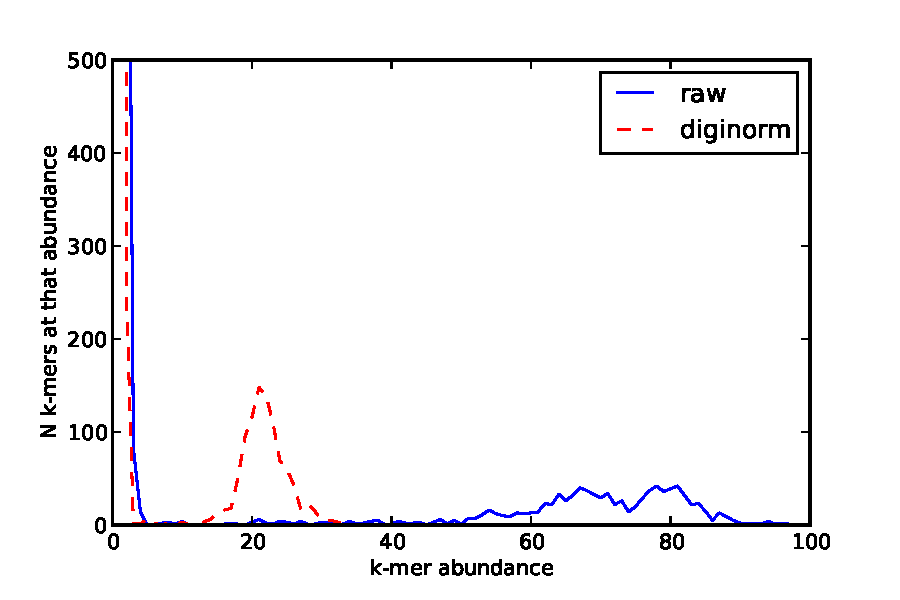
\includegraphics[width=4in]{./figures/kmer-spectrum}}
\caption{\bf K-mer spectrum of a simple artificial data set, before
  and after digital normalization.  The peaks at 1 represents
  erroneous k-mers resulting from (simulated) error; the peaks
  centered at 80 (original) and 20 (diginorm) represent k-mers truly
  present in the genome, which are shared among many reads.}
\label{fig:spectrum}
\end{figure}

% note, need to put in diginorm #s. Or do we? In Methods, maybe?

%% make compare2

\begin{table}
\begin{tabular}{|l|c|c|l|}
\hline
Name & Origin & Number of reads \\
\hline
simple genome & 10,000 & No repeats \\
{\em E. coli} MG1655 & 5,000,000 & Subset of XXXXX \\
simple transcriptome & 568 & 300:1 high:low abundance; shared exons\\
mouse mRNAseq & 1,000,000 & Subset of XXXXX \\
simple metagenome & 2,347 & 316:1 high:low abundance species  \\
mock metagenome & 5,000,000 & Subset of XXXX \\
\hline
\end{tabular}

\caption{{\bf Data sets used for evaluation.}}
\label{tab:data}
\end{table}

We next used k-mer counts from the downsampled read set to detect
errors in the original read set.  The algorithm is straightforward: we
look for bases at the beginning or ends of low-abundance runs of
k-mers in each read, which should signify the locations of errors. We
used a ``trusted k-mer'' cutoff of $C_0 = 3$ as our abundance cutoff,
below which we assumed k-mers were erroneous (see Methods).  The
results are presented in Table~\ref{tab:a}.  Of the 531 simulated
reads from the simple genome containing one or more errors, predicted
errors matched the known truth exactly for 443 of them (true
positives), and 466 reads were correctly predicted to contain no
errors (true negatives). 0 reads were falsely predicted to have no
errors (false negatives). The errors in 88 reads were miscalled --
while the reads each had one or more errors, the positions were not
correctly called -- and three reads were incorrectly predicted to
contain errors, leading to a total of 91 false positives.  From this,
we calculated the prediction sensitivity to be 100\% and the
prediction specificity to be 83.0\%.

%% make compare6
%545 erroneous reads in simple-genome-errors-nodn.pos
%531 erroneous reads in simple-genome-reads.mut.pos
%440 reads in common => all error positions AGREE
%91 DISAGREE
%total # of reads: 1000
%TP: 440
%TN: 455
%FP: 105
%FN: 0
%sensitivity: 1.0
%specificity: 0.807339449541

When we applied spectral error detection to the unnormalized reads, we
saw similar results: 440 TP, 455 TN, 105 FP, and 0 FN, for a
sensitivity of 100\% and a specificity of 80.7\% (Table~\ref{tab:a}).
(Note: for this analysis we used a cutoff of $C_0=10$.)

% @CTB here we could describe # of k-mers, etc.

\begin{table}
\begin{tabular}{|l|c|c|}
\hline
{\bf Simple genome} & Original counts & Diginorm counts \\
\hline
Perfect detection (TP) & 474 & 485 \\
No errors (TN) & 355 & 366 \\
Miscalled errors (FP) & 159 & 148 \\
Mispredicted errors (FP) & 12 & 1 \\
Missed errors (FN) & 0 & 0 \\
\hline
Sensitivity & 100\% & 100\% \\
Specificity & 73.5\% & 76.5\% \\
\hline
\end{tabular}

\caption{{\bf Results from spectral error detection on 1000 synthetic
    reads from a simulated 10kb genome, using original and digitally
    normalized reads.  The counts are the number of reads where all
    errors were detected perfectly (TP), errors were present and none
    were called (TN), one or more errors were miscalled (one type of
    FP), errors were mistakenly called in an error-free read (the
    other type of FP), and errors present in a read were missed
    (FN).}}
\label{tab:a}
\end{table}

% make ecoli_compare2.txt

\paragraph{{\em E. coli} reads:}
We next applied digital normalization and k-mer spectral error
detection to an Illumina data set from {\em E. coli} MG1655
\cite{pubmed21926975}.  In real reads, we do not know the location of
errors; to calculate likely errors, we mapped 5m untrimmed reads to
the known {\em E. coli} MG1655 genome with bowtie2 \cite{bowtie2} and
recorded mismatches between the reads and the genome.  These
mismatches were taken to be errors in the reads.  We found 8.0m errors
in 2.2m reads, for an overall error rate of 1.60\%.

We then compared the results of k-mer spectral error detection with
and without digital normalization.  We used the same parameters as on
the simulated genome ($C_0=10$ for unnormalized, $C_0=3$ for
normalized).  The results are presented in
Table~\ref{tab:ecoli_dn_counts}. Using the original counts, the
sensitivities were close between the unnormalized and normalized
predictions: using the original counts, we achieved a sensitivity of
99.8\%, versus 99.4\% using the counts from the digitally normalized
reads.  The specificities were also comparable -- 47.9\% using the original
counts, and 47.5\% using the digitally normalized counts.

% @CTB why are specificities so low?

% make ecoli_compare2.txt
% make ecoli_compare2_nodn.txt

\begin{table}
\begin{tabular}{|l|c|c|}
\hline
{\bf E. coli} & Original counts & Diginorm counts \\
\hline
Distinct k-mers         & 39,677,503 & 26,296,651 (66\%) \\
\hline
Perfect detection (TP)  & 1,042,325 & 1,030,787 \\
No errors (TN)          & 2,782,265 & 2,782,413 \\
Miscalled errors (FP)   & 1,133,049 & 1,140,148 \\
Mispredicted errors (FP)& 474       & 326       \\
Missed errors (FN)      & 2,135     & 6,574     \\
\hline
Sensitivity & 99.8\% & 99.4\% \\
Specificity & 47.9\% & 47.5\% \\
\hline
\end{tabular}

\caption{{\bf Results from spectral error detection on 5m {\em
      E. coli} reads, using k-mer counts from original and digitally
    normalized reads.}}

\label{tab:ecoli_dn_counts}
\end{table}

\begin{table}
\begin{tabular}{|l|c|c|c|c|}
\hline
Sample              & N reads & N normalized reads \\
\hline
{\em E. coli}       &    @@        & \\
\hline
\end{tabular}

\caption{{\bf Read counts for original and normalized data sets using
    a k-mer size of 20 and the specified coverage cutoff. Digital
    normalization reduces the total number of reads considered
    informative.}}
\label{tab:read_counts}
\end{table}

\begin{table}
\begin{tabular}{|l|c|c|c|c|}
\hline
Sample              & original read M & normalized read M \\
\hline
{\em E. coli}       &            & @@ \\
\hline
\end{tabular}

\caption{{\bf Unique k-mer counts for original and normalized data sets using a
  k-mer size of 20 and the specified coverage cutoff.  Digital
  normalization reduces the total number of k-mers being tracked.}}

\label{tab:kmer_counts}
\end{table}

% @@why such poor results on E. coli? repeats, or what?

\paragraph{{\em E. coli} error correction with Quake:}

% quake-ecoli-raw-cor.txt
% quake-ecoli-dn-cor.txt

\begin{table}
\begin{tabular}{|l|c|c|}
\hline
                                 & original    & diginorm \\
\hline
Total corrected reads            & 4,906,469   & 4,905,853 \\
Erroneous reads discarded        & 22,902      & 17,609 \\
Total bp                         & 450,687,634 & 450,630,551 \\
Total errors remaining           & 49,823      & 43,238 \\
Per-base error rate              & 0.011\%     & 0.010\% \\
\hline
\end{tabular}

\caption{{\bf Comparison of Quake results when run on the same {\em
      E. coli} data set, using k-mer counts from either the original
    data set (original) or the digitally normalized reads
    (diginorm).  All numbers are post-error correction; the original
    error rate was 1.60\%.}}

\label{tab:quake_ecoli}
\end{table}

While the results above suggest that simple spectral error detection
works equally well both before and after digital normalization, we
were concerned that we might lose informative reads and k-mers during
digital normalization.  To evaluate this, we used Quake to perform
error correction on the data set using the k-mer counts from the
digitally normalized reads, and compared the results to error
correction with the entire read data set.

The results of running Quake on the original data using counts from
the original and digitally normalized data are shown in
Table~\ref{tab:quake_ecoli}.  The performance was essentially the
same: Quake brought the overall error rate in the data set from 1.60\%
(8.0m errors) to 0.005\%-0.006\% (23,000 - 29,000 errors).

These results demonstrate that digitally normalized counts retain all
of the information necessary for effective error correction with
Quake, despite there being many fewer distinct k-mers
(Table~\ref{tab:kmer_counts}).

%../pipeline/quake-ecoli-dn-cor.txt      ../pipeline/quake-ecoli-raw-cor.txt
% posfile ecoli-reads.dn.cor.sam.pos: 17119 mutated reads of 4906448; 22984 mutations total
% 450630551 bp total
% overall error rate: 0.005100%
%
% posfile ecoli-reads.raw.cor.sam.pos: 22380 mutated reads of 4907082; 29135 mutations total
% 450687634 bp total
% overall error rate: 0.006465%

\subsection{Coverage-normalized data can be used to locate errors in variable
coverage shotgun sequencing data}

Digital normalization works on genomic data, with even coverage, as
well as on variable coverage data such as transcriptome and metagenome
data \cite{Brown2012, Lowe2015}. One of the drawbacks of spectral
abundance analysis is that it does not directly apply to data with
variable coverage.  For example, metagenomic or transcriptomic data
sets typically contain reads from both high-abundance and
low-abundance molecules.  This in turn leads to high coverage and low
coverage reads in the same data set. This variability in coverage
confounds naive spectral analysis for two reasons: first, erroneous
k-mers from very high abundance regions can accumulate and increase in
abundance over the threshold for trusted k-mers, thus appearing to be
correct; and second, correct reads from low coverage regions yield
k-mers below the trusted k-mer threshold that appear to be incorrect.
In practice, therefore, error analysis for metagenomic and
transcriptome data uses other approaches than direct spectral error
analysis \cite{Medvedev2011,others}.

Digital normalization uses a reference-free {\em estimator} of
per-read coverage, the median k-mer abundance within a read.  Using
this estimator, we developed a general approach that enables spectral
error analysis on variable coverage data.  We then applied this to two
synthetic data sets as well as two real data sets, a mock shotgun
metagenome and mRNAseq data from mouse.

\begin{figure}[!ht]
 \centerline{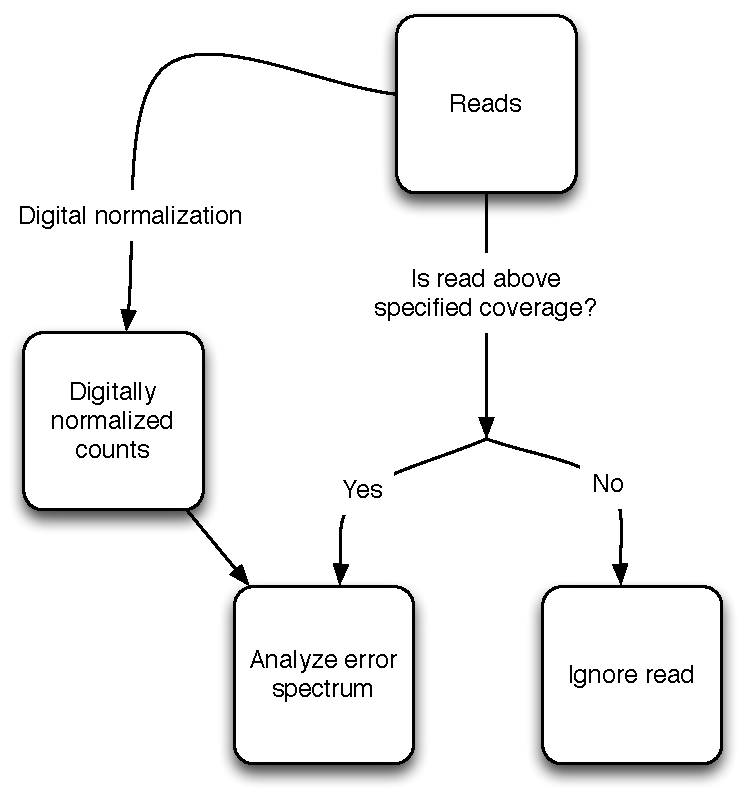
\includegraphics[width=3in]{./figures/coverage-aware-spectrum}}
\caption{{\bf Coverage-normalized spectral error analysis.  Reads are
    normalized, and high-coverage reads are subjected to spectral
    error analysis with the normalized counts, while low-coverage
    reads are ignored.}}
\label{fig:covaware}
\end{figure}

\paragraph{Coverage-normalized spectral error analysis:}

Using digital normalization, we should be able to address both the
problem of {\em too high} coverage and {\em too low} coverage.
First, by applying digital normalization to variable
coverage data and then working only with the k-mer counts from the
normalized reads, we can avoid counting high abundance errors.
Second, by ignoring reads with a low estimated coverage, we can
avoid misclassifying true low-abundance k-mers.  The process
is shown in  Figure~\ref{fig:covaware}.

% @graph with read abundance spectrum, showing which reads we will
% call errors in.

\paragraph{Simulated data:}
To test this approach, we generated two more synthetic data sets,
``simple metagenome'' and ``simple mRNAseq,'' which contain both high-
and low-abundance species (see Table~\ref{tab:data} for data set
details).  After generating synthetic reads with a 1\% error rate and
applying digital normalization (k=20/C=20), we again used the normalized
counts to do spectral error detection.  However, we used a modified
algorithm that only examined reads with a median k-mer abundance of C
or greater.

% make mcompare2
% make rcompare2

\begin{table}
\begin{tabular}{|l|c||c|}
\hline
& {\bf simple metagenome} & {\bf simple mRNAseq} \\
\hline
K-mer coverage threshold & 20 & 20 \\
Total reads & 2347 & 568 \\
High coverage reads & 2254 (96.0\%) & 524 (92.3\%) \\
\hline
Perfect detection (TP) & 978 & 228 \\
No errors (TN) & 1098 & 235 \\
Miscalled errors (FP) & 170 & 52 \\
Mispredicted errors (FP) & 6 & 9 \\
Missed errors (FN) & 2 & 0 \\
\hline
Sensitivity & 99.8\% & 100\% \\
Specificity & 84.7\% & 78.9\% \\
\hline
\end{tabular}

\caption{{\bf Variable coverage spectral error detection on two synthetic
  data sets, a simple metagenome and a simple mRNAseq data set.
  Per-read coverage was estimated by median k-mer abundance within the
  read, and only the reads with estimated coverage at or above the
  specified threshold were analyzed.  Digitally normalized counts were
  used for the spectral error analysis.}}
\label{tab:spectra_variable}
\end{table}

The results of running error detection on the synthetic metagenome and
mRNAseq data sets are shown in Table~\ref{tab:spectra_variable}. For the
simple metagenome data set, 2254 of 2347 reads (96.0\%) met the
coverage criterion.  Of the 2254 reads analyzed, the errors in 978
erroneous reads were called perfectly (TP) and 1098 of the reads with
no errors were correctly called as error-free (TN).  Only 2 reads were
incorrectly determined to be error free (FN).  Of the remaining 176
reads, 170 were miscalled (errors existed but were not exactly called)
and 6 were incorrectly called as erroneous when they were in fact
correct.  We calculated the prediction sensitivity to be 99.9\% and
the prediction specificity to be 84.7\%.  For the simple mRNAseq data
set, 524 of 568 reads (92.3\%) met the coverage criterion, with 228
true positives, 235 true negatives, 0 false negatives, and 61 false
positives, for a prediction sensitivity of 100.0\% and prediction
specificity of 78.9\%.  In neither case were low-coverage reads
included in the statistics.

Importantly, these results are comparable to the results on the
synthetic genome (100.0\% sensitivity and 83.0\% specificity with the
same parameters; see Table~\ref{tab:a}).

% make rseq_compare2

\begin{table}
\begin{tabular}{|l|c||c|}
\hline
& {\bf mouse mRNAseq} & {\bf mock metagenome} \\
\hline
K-mer coverage threshold   & 20              & 10              \\
Total reads                & 791,687         & 4,667,491       \\
High coverage reads        & 260,641 (32.9\%) & 404,896 (8.7\%) \\
\hline
Perfect detection (TP)     & 90,954          & 11,743          \\
No errors (TN)             & 141,009         & 366,253         \\
Miscalled errors (FP)      & 20,547          & 3,911           \\
Mispredicted errors (FP)   & 1173            & 21,750          \\
Missed errors (FN)         & 6931            & 1239            \\
\hline
Sensitivity                & 92.9\%          & 90.5\%          \\
Specificity                & 80.7\%          & 31.4\%          \\
\hline
\end{tabular}

\caption{{\bf The results of variable coverage spectral error detection on
  two real variable coverage data sets, a mock shotgun metagenome and
  a mouse mRNAseq data set. Per-read coverage was estimated by median
  k-mer abundance within the read, and only the reads with estimated
  coverage at or above the specified threshold were analyzed.
  Digitally normalized counts were used for the spectral error analysis.}}
\label{tab:spectra_variable_real}

\end{table}

\paragraph{mRNAseq data:}

% rseq_compare2.txt

To evaluate coverage-normalized spectral analysis on real data, we
applied variable coverage spectral error analysis to 1m mouse mRNAseq
reads \cite{Haas2013}.  After calling errors in the reads by mapping
them back to the known genomes, we used spectral analysis to identify
putative errors.  The results are shown in
Table~\ref{tab:spectra_variable_real}, third column.  We achieved
92.9\% sensitivity and 80.7\% specificity on the 340,000 high coverage
reads in this data set.

\paragraph{Mock metagenome data:}

% podar_compare2.txt

We next applied our approach to 5m reads from a diverse mock community
data set (Shakya et al., 2013). We used a coverage threshold of 10 for
digital normalization, and found that 404,896 reads were at or above
this coverage threshold.  Here errors were again calculated by mapping
the reads to the known reference and finding mismatches.  The results
are shown in Table~\ref{tab:spectra_variable_real}, second column.  We
achieve 90.5\% sensitivity and 41.4\% specificity on the high coverage
reads; here, the poor specificity is probably due to the modified coverage
cutoff needed for this low coverage subset of the high diversity
mock metagenome (discussed below).

\paragraph{Error correcting variable coverage data with Quake:}

% rseq_compare6.txt

There are many sophisticated error correction algorithms implemented
for shotgun genome data, but relatively few work directly on variable
coverage data such as mRNAseq.  Digital normalization, in theory,
enables the use of {\em any} genomic error correction algorithm on the
high coverage components of data sets.

To evaluate this, we used Quake (a genomic error corrector) to correct
the high coverage mRNAseq reads using the diginorm counts.  We first
extracted the 260,641 reads with estimated coverage greater than or
equal to 20 from the mouse mRNAseq data set, and then digitally
normalized the data.  We next applied the Quake error corrector to the
unnormalized high-coverage reads using the k-mer counts from the
normalized reads, as with the {\em E. coli} data set.  Quake discarded
23,606 reads and corrected the remainder.

% quake-ecoli-raw-cor.txt
% quake-ecoli-dn-cor.txt

\begin{table}
\begin{tabular}{|l|c|}
\hline
{\bf mRNAseq}                    & diginorm \\
\hline
Total reads                      & 791,687 \\
High coverage reads              & 260,641 \\
Erroneous reads discarded        & 23,606 \\
Total bp after correction        & 17,254,585 \\
Total errors remaining           & 74,797 \\
Per-base error rate              & 0.43\% \\
\hline
\end{tabular}

\caption{{\bf Results of running Quake on mRNAseq. @@@ Comparison of Quake results when run on the same {\em
      E. coli} data set, using k-mer counts from either the original
    data set (original) or the digitally normalized reads
    (diginorm).  All numbers are post-error correction; the original
    error rate was 1.60\%.}}

\label{tab:quake_mrna}
\end{table}

We evaluated the corrected reads by mapping them against the mouse
transcriptome, and found that, for the retained reads, Quake reduced
the overall error rate from 1.28\% (230,125 mismatches in 18,012,456
bp total) to 0.43\% (74,797 in 17,254,585 total) - see
Table~\ref{tab:quake_mrna}.  As with {\em E. coli}, this suggests that
sufficient information remains in the digitally normalized data to do
an effective job of error correction.

\subsection{A streaming algorithm can be used for spectral error analysis}

The spectral error detection approach outlined above is a 2-pass
offline algorithm for any given data set - the first pass normalizes
the read set and records the k-mer abundances, while the second pass
analyzes the reads for low-abundance k-mers.  Even with digital
normalization reducing the number of k-mers under consideration, this
2-pass approach is time consuming on large data sets.  Below, we
develop a general streaming approach that considers many of the
reads only once.

\paragraph{Streaming analysis of coverage-saturated regions:}

Shotgun sequencing oversamples most regions -- for example, for a 100x
coverage genomic data set, we would expect 50\% or more of the genome
to be represented by more than 100 reads.  This is a consequence of
the Poisson-random sampling that underlies shotgun sequencing \cite{Waterman}.
This oversampling provides an opportunity, however: if we
regard the read data set as a stream of incoming data randomly sampled
from a pool of molecules, high-abundance species or subsequences
within the pool will be more highly sampled in the stream than others,
and will thus generally appear earlier in the stream.  For example, in
mRNAseq, highly expressed transcripts will on average be highly
sampled much more frequently than low-expressed transcripts, and more
reads from highly expressed transcripts will be seen in any given
subset.

We can adapt the same approaches used in previous sections to do {\em
  streaming} error analysis by detecting and analyzing high-coverage
reads {\em during} the first pass.  Here we again use the median k-mer
abundance within a read to estimate read coverage \cite{Brown2012};
crucially, this can be done at any point in a stream, by using the
online k-mer counting functionality of khmer to determine the
abundance of k-mers seen thus far in the stream \cite{Zhang2014}.

The conceptual idea is presented in Figure~\ref{fig:concept}.  On the
first pass, low-coverage reads would be incorporated into the k-mer
database and set aside for later analysis, while high-coverage reads
would be analyzed for errors. On the second pass, the set aside reads
would be checked for coverage again, and either ignored or analyzed
for errors.  Crucially, this second pass involves {\em at most}
another full pass across the data, but only when the entire data set
is below the coverage threshold; the larger the high coverage
component of the data, the smaller the fraction of the data that is
examined twice.

\begin{figure}[!ht]
 \centerline{\includegraphics[width=4in]{./figures/graph-saturation}}
\caption{\bf Diagram of streaming error detection. In a first pass
over the read data, reads are loaded in until the graph locus to which
they belong is saturated.  From that point on, reads are examined for
errors and not loaded into the graph.  In a second pass, only the subset
of reads loaded into the graph are examined for errors.}
\label{fig:concept}
\end{figure}

In Figure~\ref{fig:saturation}, we show diginorm-generated coverage
saturation curves for both real and error-free simulated reads from
{\em E. coli} MG1655.  In both cases, after the first 1m reads, the
majority of reads have an estimated coverage of 20 or higher, and
hence can be used for error analysis on the first pass through the
data.

\begin{figure}[!ht]
 \centerline{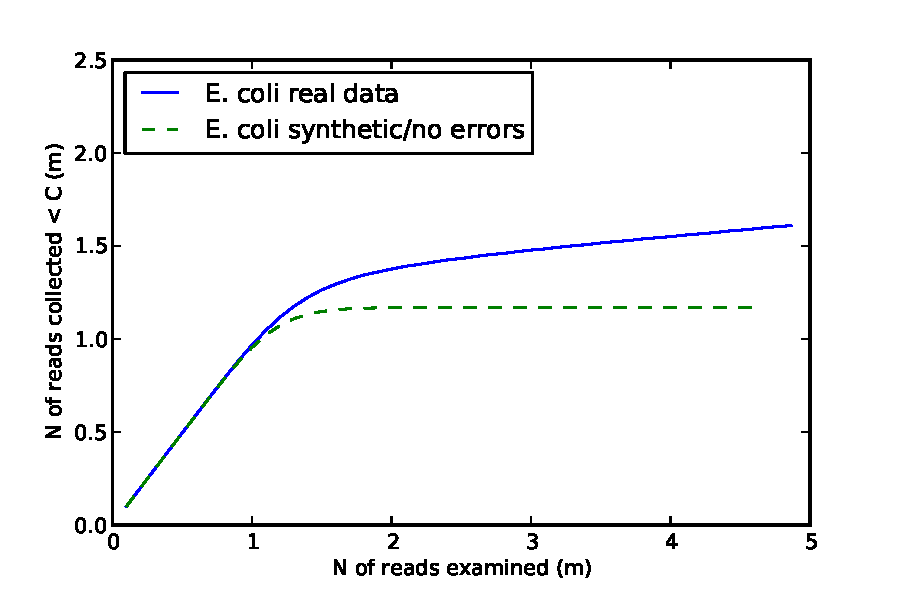
\includegraphics[width=4in]{./figures/saturation}}
\caption{\bf Saturation curve of a real and a simulated {\em E. coli}
  read data set.  Reads are collected when they have an estimated
  coverage of less than 20; in the early phase ($<$ 1m reads), almost
  all reads are collected, but by 2m reads into the data set, the
  majority of reads come from loci with an estimated sequencing depth
  of $>$ 20 and are rejected.}
\label{fig:saturation}
\end{figure}

% make compare4
% make mcompare4
% make rcompare4

\begin{table}
\begin{tabular}{|l|c||c||c|}
\hline
& {\bf simple genome} & {\bf simple metagenome} & {\bf simple mRNAseq} \\
\hline
Number of passes & 1.32 & 1.16 & 1.33 \\
\hline
Perfect detection (TP) & 485 & 977 (-1) & 228 \\
No errors (TN) & 365 (-1) & 1095 (-3) & 235 \\
Miscalled errors (FP) & 148 & 171 (+1) & 52 \\
Mispredicted errors (FP) & 2 (+1) & 9 (+3) & 9 \\
Missed errors (FN) & 0 & 2 & 0 \\
\hline
Sensitivity & 100.0\% & 99.9\% & 100.0\% \\
Specificity & 76.4\% & 84.4\% & 78.9\% \\
\hline
\end{tabular}
\caption{{\bf Results from applying streaming error detection to the
    same synthetic data sets as in Table~\ref{tab:a} and
    Table~\ref{tab:spectra_variable}.  Number of passes is the average
    number of times each read in the data set was examined; numbers in
    parentheses give the difference between these numbers and the
    previous results.}}
\label{tab:spectra_streaming}

\end{table}

Moreover, because only the normalized counts are used in spectral
analysis, the approach should apply equally well to data sets with
uneven coverage, i.e. metagenomes and transcriptomes.  To test this,
we first apply this streaming error detection approach to the three
synthetic data sets used earlier, and then to the three real data
sets.

\paragraph{Streaming error analysis of synthetic data:}

Using the streaming approach on the ``simple genome'' reads, we obtain
nearly identical numbers to the full two-pass approach: 485 TP, 365
TN, 150 FP, and 0 FN, for a sensitivity of 100\% and a specificity of
76.3\% (Table~\ref{tab:spectra_streaming}).  However, with the
streaming algorithm, only 320 of the 1000 reads are examined twice.
Likewise, for the ``simple mRNAseq'' and ``simple metagenome'' data
sets, we obtain identical and nearly identical results, respectively;
due to differences in the order in which reads are examined, the
simple metagenome fails to detect one true positive and erroneously
finds errors in three extra reads.  On the mRNAseq data set, 33.1\% of
the reads are examined twice, and on the metagenome, 380 of 2347
(16.2\%) of the reads are examined twice.

\paragraph{Streaming error analysis of real data:}

% ecoli_compare4.txt

% rseq_compare4.txt

% podar_compare4.txt

\begin{table}
\begin{tabular}{|l|c||c||c|}
\hline
& {\bf \em E. coli} & {\bf mouse mRNAseq} & {\bf mock metagenome} \\
\hline
Number of passes & xx & yy & zz \\
\hline
Perfect detection (TP)   & 1,033,261 & 91,133  & 11,726  \\
No errors (TN)           & 2,781,961 & 140,461 & 364,627 \\
Miscalled errors (FP)    & 1,138,940 & 20,741  & 3,951   \\
Mispredicted errors (FP) & 778       & 1721    & 23,376  \\
Missed errors (FN)       & 5308      & 6584    & 1216    \\
\hline
Sensitivity            & 99.5\%      & 93.3\%  & 90.6\%  \\
Specificity            & 47.6\%      & 80.2\%  & 30.0\%  \\
\hline
\end{tabular}
\caption{{\bf Results from applying streaming error detection to the same
  real data sets as in Table~\ref{tab:ecoli_dn_counts} and
  Table~\ref{tab:spectra_variable_real}.  Number of passes is the average
  number of times each read in the data set was examined; unless noted in
  parentheses, numbers were within 1\% of non-streaming results.}}
\label{tab:spectra_streaming_real}

\end{table}

We also get similar quality results on the real data sets when
comparing two-pass error detection with streaming error detection
(Table~\ref{tab:spectra_streaming_real}).  For {\em E. coli}, with
streaming error detection we obtain a sensitivity of 99.5\% and a
specificity of 47.6\%, compared to 99.8\% and 47.9\% with the two-pass
approach (Table~\ref{tab:ecoli_dn_counts}).  For the mock metagenome,
we have a sensitivity of 90.6\% with streaming, vs 90.5\% with the
two-pass approach; and a specificity of 30.0\% with streaming, vs
31.4\% with the two pass approach (compare
Table~\ref{tab:spectra_streaming_real} and
Table~\ref{tab:spectra_variable_real}).  And for the mRNAseq data set,
we see a sensitivity of 93.3\% with streaming vs 92.9\% with two-pass,
and a specificity of 80.2\% vs 80.7\% for streaming vs two-pass,
respectively.  However, the streaming
approach examined the {\em E. coli} reads only XX times, the
metagenome reads YY times, and the mRNAseq reads ZZ times on average.

\subsection{A streaming algorithm can be used for error trimming}

Once errors can be {\em detected} with a streaming algorithm, errors
can also be {\em removed} by trimming reads at the first base
predicted to be erroneous in a read.  This approach is remarkably
effective, but can require considerably more memory than quality-score
based trimming \cite{Zhang2014}.  Moreover, it is currently
implemented as an offline (two-pass) algorithm.  Below, we apply the same
streaming approach shown in Figure~\ref{fig:concept} to trimming
reads.

%  (While it is possible to split reads around errors
%rather than truncating them, this introduces complications in
% downstream read processing.)

% make compare5

\paragraph{Streaming error trimming on synthetic data:}

On the ``simple genome'' with counts from the digitally normalized
reads, this trimming approach eliminates 149 reads entirely and
truncates another 392 reads.  Of the 100,000 bp in the simulated
reads, 31,910 (31.9\%) were removed by the trimming process.  In
exchange, trimming eliminated {\em all} of the errors, bringing the
overall error rate from 0.63\% to 0.00\%.

% make mcompare5
% make rcompare5

For the simple metagenome we used the variable abundance approach
described above and only trimmed reads with estimated coverage of 20
or higher.  Here, of 2347 reads containing 234,700 bp, 314 reads
(13.4\%) were removed and 851 reads (36.3\%) were trimmed, discarding
a total of 74,321 bases (31.7\%).  Of 1451 errors total, all but 61
were eliminated, bringing the overall per-base error rate from 0.62\% to
0.04\%.  The simple mRNAseq data set showed similar improvement: 83 of
568 reads were removed, and 208 were trimmed, removing 19,507 of
56,800 bases (34.34\%).  The initial error rate was 0.65\% and the
final error rate was 0.07\%.

\begin{table}
\begin{tabular}{|l|c|c|c|c|}
\hline
Data set        & pre-trim error & \% bp trim & \% reads trim & post-trim error \\
\hline
{\em E. coli}   & 1.60\%         &                  &             & 0.05\% \\
Mock metagenome & 0.32\%         &                  &             & 0.30\% \\
mouse mRNAseq   & 2.07\%         &                  &             & 1.84\% \\
(high coverage only) & 1.61\%    &                  &             & 0.66\% \\
mock metagenome &                &                  &             &        \\
(high coverage only) &           &    @@              &             &        \\
\hline
\end{tabular}

\caption{{\bf A summary of trimming statistics for streaming error trimming.
Error rates before and after trimming were estimated by mapping mismatches.}}
\label{tab:trimming}
\end{table}

\paragraph{Streaming error trimming on real data:}

% ecoli-report-untrim.txt ('make ecoli-report-untrim.txt')
%posfile ecoli-reads.sam.pos: 2177509 mutated reads of 4960248; 7990149 mutations total
%496024800 bp total
%overall error rate: 1.610837%

% ecoli-report-trim.txt ('make ecoli-report-trim.txt')
%posfile ecoli-abundtrim.sam.pos: 164655 mutated reads of 4861345; 203345 mutations total
%434621201 bp total
%overall error rate: 0.046787%

% output of 'make ecoli-mapped.fq.gz.abundtrim'
%
% read 4960248 reads, 496024800 bp
% wrote 4861345 reads, 434621201 bp
% removed 98903 reads and trimmed 2030456 reads
% trimmed or removed 12.38% of bases (61403599 total)
% fp rate estimated to be 0.004

Applying the streaming error trimming to the {\em E. coli} MG1655 data
set used in section XXX, we trimmed 2.0m reads and removed 98,903
reads entirely.  Of 8.0m errors, all but 203,345 were removed,
bringing the error rate from 1.60\% to 0.05\%.  Trimming discarded 61
Mbp of the original 500 Mbp (12.4\%).

% output of 'make rseq-mapped.fq.gz.abundtrim'
%
% read 791687 reads, 60168212 bp
% wrote 763468 reads, 56846899 bp
% removed 28219 reads and trimmed 70260 reads
% looked at 617297 reads twice
% trimmed or removed 5.52% of bases (3321313 total)
% skipped 531046 reads/40359496 bases because of low coverage

% rseq_compare5.txt
% rseq_compare5b.txt

% output of 'make podar-mapped.fq.gz.abundtrim'
% 
% read 4667491 reads, 471416591 bp
% wrote 4661668 reads, 470184476 bp
% removed 5823 reads and trimmed 21231 reads
% looked at 4565119 reads twice
% trimmed or removed 0.26% of bases (1232115 total)
% skipped 4262595 reads/430522095 bases because of low coverage

% make podar_compare5

On the mouse mRNAseq data set, streaming error trimming removed 28,219
reads and trimmed 70,260 reads, removing 5.52\% of the total bases,
bringing the overall error rate from 2.1\% to 1.8\%.  When we measured
only the error rate in the high-coverage reads, trimming brought the
error rate from 1.61\% to 0.66\%.  On the mock metagenome data set,
5823 reads were removed and 21,231 reads were trimmed, removing 0.26\%
of bases; this low percentage is because of the very low coverage of
most of the reads in this data set.  XXX

\subsection{Illumina error rates and error profiles can be determined from a
small sample of sequencing data}

\begin{figure}[!ht]
 \centerline{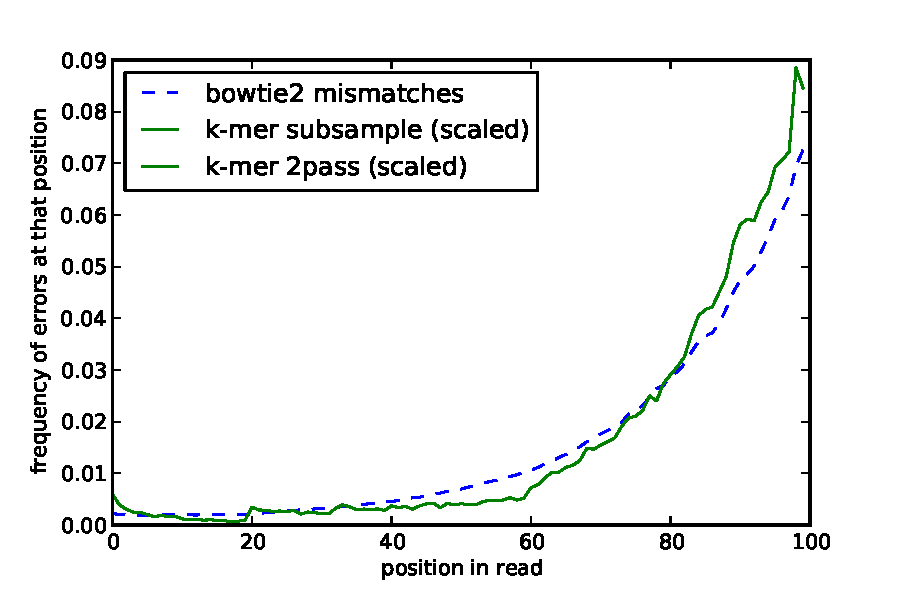
\includegraphics[width=4in]{./figures/ecoli-errhist}}
\caption{{\bf Error spectrum of reads in the {\em E. coli} data
    set. The sublinear k-mer spectrum analysis is calculated based on
    saturation of a fraction of the data set, while the two-pass
    spectral analysis uses all of the data.  bowtie2 mismatches are
    based on all mapped reads.  The y values for the k-mer spectral
    analyses are scaled by a factor of four for ease of comparison.}}
\label{fig:ecoli_err}
\end{figure}

\begin{figure}[!ht]
 \centerline{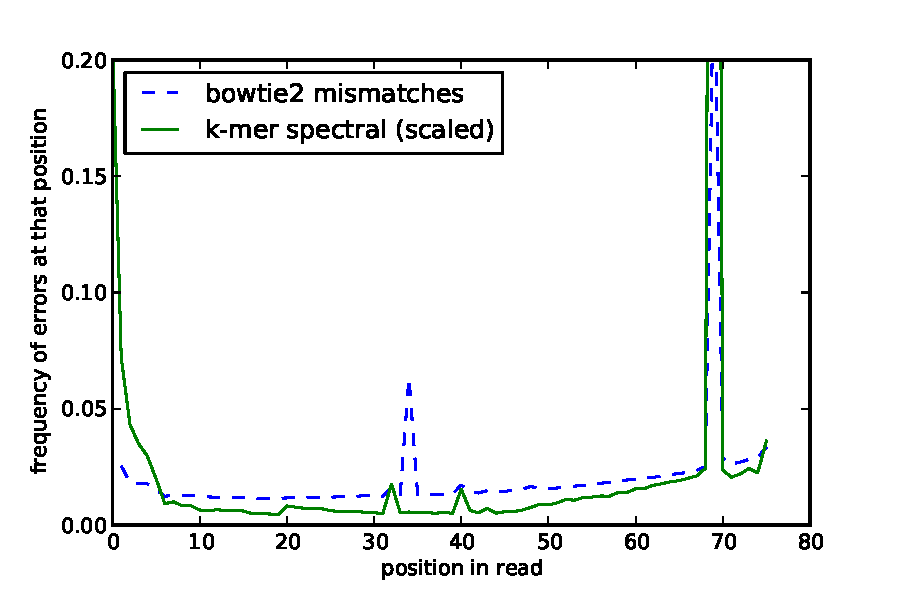
\includegraphics[width=4in]{./figures/rseq-errhist}}
\caption{{\bf Error spectrum of reads in the mouse RNAseq data set.
    The sublinear k-mer spectrum analysis is calculated based on
    saturation of a fraction of the data set, while the two-pass
    spectral analysis uses all of the data, and bowtie2 mismatches are
    based on all mapped reads.  The peak of errors at position 34 in
    the bowtie2 mapping reflects errors that in the first part of the
    data set are called as Ns, and hence are ignored by the sublinear
    error analysis; see text for details. Note, the bowtie2 mismatch
    rates are larger than the spectral rates, so for ease of
    comparison the y values for the k-mer spectral analyses are scaled
    by a factor of four.}}
\label{fig:rseq_err}
\end{figure}

With Illumina sequencing, average and per-position error rates may
vary between sequencing runs, but are typically systematic within a
run \cite{drisee,XXX}.  Melsted and Halldorson (2014) introduced an
efficient streaming approach to estimating per-run sequencing error,
but this approach does not apply to error rates by position within
reads.  Here, k-mer spectral error analysis can be used to calculate
per-position relative sequencing error for entire data sets
\cite{Zhang2014}.

We can adapt the streaming approaches above to efficiently provide
estimates for {\em subsets} of the data.  The basic idea is to consume
reads until sufficient data has been collected to calculate error
rates, and then to calculate error rates for new reads based on the
k-mer abundances from the consumed reads.  This can be done in one
pass for data sets with sufficiently high coverage data: as shown
above (Figure~\ref{fig:saturation}), in some data sets, most of the
reads will have sufficient coverage to call errors by the time 20\% of
the data set has been consumed.

Using the same error detection code as above, we implemented a
sublinear memory/sublinear time algorithm that collects reads until
some regions have reached 20x coverage, or 200,000 reads have
surpassed a coverage of 10x (see Methods for details).  In either
case, all reads at or above a coverage of 10 are analyzed for errors,
with a trusted k-mer cutoff of 3.  In Figure~\ref{fig:ecoli_err} and
Figure~\ref{fig:rseq_err} we show the resulting error profiles for the
{\em E. coli} and mouse RNAseq data sets, compared with the profile
obtained by examining the locations of mismatches to the references.
We also show the error profile obtained with the full two-pass approach
(using digital normalization and then error detection as in section XXX)
for comparison.

In the {\em E. coli} data set (Figure~\ref{fig:ecoli_err}), we see the
increase in error rate towards the 3' end of the gene that is
characteristic of Illumina sequencing (cite).  All three error
profiles agree in shape (Pearson's correlation of 0.99 between each
pair) although they are offset considerably in absolute magnitude.
The k-mer error profile was calculated from the first XXX reads, but
is consistent across five other subsets of the data chosen randomly
with reservoir sampling (data not shown); all five subsets had
Pearson's correlation coefficients greater than 0.99 with the
bowtie2 mapping profile and the two-pass spectral approach.

The RNAseq error profile exhibits two large spikes, one at position 34
and one at position 69.  Both spikes appear to be genuine and
correlate with large numbers of Ns in those positions in the original
data set.  The spikes are present in the profiles derived from
two-pass spectral analysis as well as the bowtie2 mismatch
calculation.  However, the sublinear approach does not detect them
when using the first YYY reads.  This is because of the choice of
subsample: five other subsamples, chosen randomly from the entire data
set with reservoir sampling, match the match the two-pass spectral
analysis (data not shown).  The error profiles calculated from all six
subsamples with the sublinear algorithm have a Pearson's correlation
coefficient greater than 0.96 with the error profiles from the full
two-pass spectral approach and the bowtie2 mismatches.

% @CTb discuss subsample in discussion

\subsection{Time and space considerations}

The digital normalization algorithm is, in Python pseudocode:
\begin{verbatim}
for read in data:
   if coverage(read, table) < DESIRED:
      add_read_to_table(read, table)
      save(read)
\end{verbatim}
This is a single-pass algorithm that, if at least one read has
coverage equal to or greater than {\tt DESIRED}, is sublinear in
space \cite{Brown2012}.  (Technically, that read must also have
an error, if {\tt table} is counting k-mers.)  In practice, for data
sets with an average coverage higher than {\tt DESIRED}, the majority
of individual reads will not be collected (see Figure~\ref{fig:saturation}).

The modifications to the algorithm for {\em streaming} are as follows:
\begin{verbatim}
for read in data:  # first pass
   if coverage(read, table) < DESIRED:
      add_read_to_table(read, table)
      save(read)
   else:
      analyze(read)

for read in saved_reads:   # second pass
   if coverage(read, table) >= DESIRED:
      analyze(read)
\end{verbatim}

Here, the space used remains identical to the digital normalization
algorithm and is hence sublinear in high coverage data sets, but the
algorithm is no longer single-pass.  However, in any high coverage
data set, some reads will {\em not} be saved, and the second pass
across the saved data is guaranteed to be less than a full pass, and
hence the total number of passes will be less than two.  Graphically,
any deviation from the identity line in a saturation analysis as in
Figure~\ref{fig:saturation} yields a few-pass algorithm.

\subsection{Performance on full mRNAseq and metagenomic data sets}

In practice, the space and memory performance of both digital
normalization and the generalized streaming approach presented here
depend on specific details of the data set under analysis and the
precise implementation of the coverage estimator. While our intention
in this paper is to demonstrate the general streaming approach, we
note that even our naive implementation for e.g. streaming trimming is
useful and can be applied to very large data sets.  For high coverage
data, we can efficiently error-trim 10s of millions of reads in both
sublinear memory and fewer than two passes acros the data.  In
Table~\ref{tab:full_trimming}, we show the summary statistics for
streaming error trimming of the full mouse mRNAseq and mock metagenome
data; in contrast to the smaller subsets used previously (see
Table~\ref{tab:trimming}), when we consider the full data sets the
majority of reads are examined only once (see ``Number of passes'',
Table~\ref{tab:full_trimming}).

\begin{table}
\begin{tabular}{|l|c|c|c|c|}
\hline

Data set             & mouse mRNAseq      & mock metagenome \\
Coverage cutoff      & 20                 & 10 \\
\hline
Total reads          & 36,882,401         & 50,328,673 \\
Total bp             & 2,803,062,476      & 5,083,195,973 \\
High-coverage reads  & 33,451,281         & 35,753,645 \\
Number of passes     & 1.23               & 1.29 \\
\% reads trim        & 27\%               & 5\% \\
\% bp trim           & 17.82\%            & 2.3\% \\
Pre-trim error rate  & 1.24\%             & 0.28\% \\
Post-trim error rate & 0.73\%             & 0.17\% \\
\hline
\end{tabular}

\caption{{\bf Results of streaming error trimming on complete data sets.
Error rates before and after trimming were estimated by mapping mismatches.}}
\label{tab:full_trimming}
\end{table}

\section{Discussion}

\subsection{Digital normalization can be applied effectively to short reads prior to error detection and correction.}

Tracking k-mer abundances in large short-read data sets is part of
many error detection and correction algorithms, but this process can
be time and memory intensive.  Here we show that for some data sets,
digital normalization can be used to reduce the total number of k-mers
under consideration without strongly affecting results.
We showed this in both simulated and real data.

With a real {\em E. coli} data set, digital normalization reduced the
number of k-mers by a third (Table~\ref{tab:ecoli_dn_counts}, Distinct
k-mers) yielding essentially the same sensitivity and specificity of
error predictions.  Moreover, when we ran the Quake error corrector on
the reads using unnormalized and normalized counts
(Table~\ref{tab:quake_ecoli}), we achieved nearly identical results,
demonstrating that the digital normalized data set retained all of the
information necessary for error correction.

\subsection{K-mer counts from digitally normalized short reads can be used to error correct mRNAseq and metagenome data}

Spectral error correction approaches typically rely on assumptions of
uniform sequence coverage, but these assumptions are violated by
several types of data, including mRNAseq and shotgun metagenome data.
Digital normalization evens out this coverage, allowing existing
spectral error correction approaches to be applied to data from
samples with non-uniform abundances.  We demonstrated this by using
spectral error detection with digitally normalized data to predict
errors in both synthetic and real RNAseq and metagenome data
(Table~\ref{tab:spectra_variable_real}).  We then again used Quake to
error correct high-coverage portions of mRNAseq and shotgun metagenome
data sets, which yielded promising results
(Table~\ref{tab:quake_mrna}).  This again demonstrates that digitally
normalized data retains the information necessary to error correct
high coverage reads.

It is not clear how widely applicable diginorm is as a pre-processor
for k-mer spectral analyses: here we used only three real data sets,
with one set of diginorm parameters.  Absent a theoretical
understanding of digital normalization, we cannot extend these results
to all short-read data sets nor can we predict which parameter
combinations will succeed.  However, with these parameters, digital
normalization retains the vast majority of ``true'' k-mers in several
data sets \cite{Brown2012}, which speaks directly to the basis of
k-mer spectral analysis.  In addition, digital normalization and
derivative approaches have proven to be fairly robust in leading to
good assemblies with genomic data, RNAseq data, single-cell data, and
metagenome data \cite{Brown2012,Lowe2015,Howe2014}.  We are therefore
hopeful that this will prove to be a general practical approach.

% @  (Comment on adaptation of existing
% err corr, e.g. Lighter?)

\subsection{Short-read error detection and trimming can be done efficiently with a streaming few-pass sublinear-memory algorithm}

K-mer spectral error detection, trimming, and correction approaches
are typically implemented as a two-pass offline algorithm, in which
k-mer counts are collected in a first pass and then reads are
corrected in a second pass.  While several algorithms that run in sub
linear memory do exist (e.g. Lighter), these are still offline
algorithms that require at least two full passes across the data.

In high coverage data sets it is possible to implement a more
algorithmically efficient approach, by detecting reads that are high
coverage in the context of reads previously encountered in the same
pass of the data.  We implemented this by integrating k-mer spectral
error analysis directly into the digital normalization algorithm, and
showed that on several synthetic and real data sets, we achieved
nearly identical predictions to the full two-pass algorithm with an
algorithm that is less than two pass (compare
Table~\ref{tab:spectra_variable_real} to
Table~\ref{tab:spectra_streaming_real}).

We also adapted the error detection algorithm to do streaming error
trimming on genomic, metagenomic, and transcriptomic data.  On high
coverage components of variable coverage data sets, this led to
a substantial decrease in errors - up to an order of magnitude.
(XXX Talk about large, real data sets - Sherine work.)

As with digital normalization, a basic streaming approach is very
simple to implement: given an online way to count k-mers, the
algorithm is approximately 10 lines of Python code.  The approach also
requires very few parameter choices: the only two parameters are k-mer
size and target coverage.  However, we do not yet know how these
parameters interact with read length, error rate, or data set
coverage; systematic evaluation of parameters and the development of
underlying theory is left for future work.

The implementation of streaming error trimming used in this paper is
somewhat inefficient, and relies on redundantly storing all of the
reads needed for the second pass on disk during the first pass.  In
the worst case (discussed below) a complete copy of the data set may
need to be stored on disk!  This is an area for future improvement.

\subsection{Data-set wide error profiles can be calculated in sub linear time and memory}

The ability to analyze high-coverage reads without examining the
entire data set offers some intriguing possibilities.  One concrete
application is the use of high coverage reads to infer data-set wide
error characteristics for shotgun data, in a way that is robust to the
sample.  Can also be used to assess whether the necessary coverage has
been obtained in order to truncate sequencing, in e.g. metagenomics
workflows.

More generally, the approach of using saturating coverage to truncate
computational analysis may have application to streaming sequencing
technologies such as Nanopore, where realtime feedback between
sequencing and sequence analysis could be useful.

\subsection{Worst-case and best-case scenarios: when is streaming error
trimming best applied?}

Here we introduce an approach to removing erroneous k-mers from large
sequencing data sets with a streaming algorithm that takes into
account variable coverage data sets.  When should this be applied?

The general streaming algorithm is most time-efficient on data sets
where most of the data is high coverage, because the second pass
across the data is limited to the set of reads that is low coverage on
the first pass (Figure~\ref{fig:concept}).  Even though the coverage
of the data sets may not be known in advance, the approach is robust
to low-coverage data: low-coverage reads will simply be ignored by any
approach based.

One particularly appealing aspect of the variable coverage error
trimming approach is that it does not need to be modified for
different data sets: the underlying algorithm can be applied equally
to genomic, mRNAseq, and metagenome data sets, although read lengths,
error rates, and data set coverage will affect the quality of results.
On high coverage genomic data sets, trimming can be made more
stringent by eliminating all low-abundance k-mers as erroneous, but
even if this is not done, the underlying approach is equally
efficient.

Digital normalization was developed primarily to decrease the memory
requirements for De Bruijn graph assembly by eliminating erroneous
k-mers; diginorm can reduce the memory requirements for Velvet by more
than an order of magnitude.  However, diginorm also alters the
coverage of the data set, which may affect the performance of
assemblers or other downstream analysis steps that rely on coverage.
While streaming error trimming removes at least as many k-mers as
digital normalization (and generally should remove many more), k-mer
based error trimming should have a much smaller effect on data set
coverage.  Moreover, trimming generally eliminates far less of the
data set than digital normalization.  This may make trimming a more
palatable pre-filter for assembly than digital normalization.

We would caution against using variable coverage error trimming before
mapping-based abundance analyses such as transcript quantification,
ChIP-seq, or variant calling.  Variable coverage error trimming
preferentially retains low-abundance reads and eliminates portions of
high abundance reads, which may bias results.

\subsection{Concluding thoughts}

We describe time- and memory- efficient general algorithmic approaches
to k-mer spectral error detection and correction based on read-local
analysis of coverage.

These approaches can be applied to variable coverage data, including
mRNAseq and shotgun metagenome reads.

Future applications include streaming error correction, reference-free
variant calling, and reference-free analysis of streaming sequencing
data.

\bibliography{2014-streaming}

\end{document}
